\documentclass[letterpaper,9pt,twocolumn,twoside,]{pinp}

%% Some pieces required from the pandoc template
\providecommand{\tightlist}{%
  \setlength{\itemsep}{0pt}\setlength{\parskip}{0pt}}

% Use the lineno option to display guide line numbers if required.
% Note that the use of elements such as single-column equations
% may affect the guide line number alignment.

\usepackage[T1]{fontenc}
\usepackage[utf8]{inputenc}

% pinp change: the geometry package layout settings need to be set here, not in pinp.cls
\geometry{layoutsize={0.95588\paperwidth,0.98864\paperheight},%
  layouthoffset=0.02206\paperwidth, layoutvoffset=0.00568\paperheight}

\definecolor{pinpblue}{HTML}{185FAF}  % imagecolorpicker on blue for new R logo
\definecolor{pnasbluetext}{RGB}{101,0,0} %



\title{An Abalone-Age Investigation}

\author[]{\textbar{} 470408957 \textbar{} 480423142 \textbar{} 490209370
\textbar{} 490384806 \textbar{} 490443251 \textbar{}}


\setcounter{secnumdepth}{3}

% Please give the surname of the lead author for the running footer
\leadauthor{}

% Keywords are not mandatory, but authors are strongly encouraged to provide them. If provided, please include two to five keywords, separated by the pipe symbol, e.g:
 

\begin{abstract}
In this report, we investigate whether the age of \emph{Haliotis}
\emph{Rubra} \emph{(Blacklip} \emph{Abalone)} can be estimated from
external physical attributes. We constructed and evaluated two multiple
linear regression models using the Akaike Information Criterion (AIC).
After refinement of the selected model, we found that given two weights,
three dimensions, and the sexual maturity of an abalone, we could
explain 62.8\% of the the variance in our target variable. Provided
these measurements, predictions could in turn be untransformed to
generate age estimates for abalone.
\end{abstract}

\dates{Data2002 Group Project \textbar{} November 2020}


% initially we use doi so keep for backwards compatibility
% new name is doi_footer
\doifooter{\url{https://github.sydney.edu.au/jary8982/M09B_early_5.git}}

\pinpfootercontents{Data2002 Group Project}

\begin{document}

% Optional adjustment to line up main text (after abstract) of first page with line numbers, when using both lineno and twocolumn options.
% You should only change this length when you've finalised the article contents.
\verticaladjustment{-2pt}

\maketitle
\thispagestyle{firststyle}
\ifthenelse{\boolean{shortarticle}}{\ifthenelse{\boolean{singlecolumn}}{\abscontentformatted}{\abscontent}}{}

% If your first paragraph (i.e. with the \dropcap) contains a list environment (quote, quotation, theorem, definition, enumerate, itemize...), the line after the list may have some extra indentation. If this is the case, add \parshape=0 to the end of the list environment.


\hypertarget{introduction}{%
\section{Introduction}\label{introduction}}

Marine biologists and conservationists often study the age and growth
patterns of a species in order to understand its demographics in and
across various ecosystems. As a sought after commodity within the
fishing industry, this is especially true of Abalone. However, the
classical method for determining an abalone's age is arduous and time
inefficient; counting the rings in a specially prepared shell under a
microscope (\cite{Dua:2019}). We therefore aim to find a technique for
estimating an abalone's age using only physical attributes which are
easily and quickly measured. We will construct a multiple regression
model in order to predict the number of rings an abalone has, and
evaluate whether this model can effectively predict observed values and
would therefore have any utility when applied to new observations.

\hypertarget{data-set}{%
\section{Data Set}\label{data-set}}

This data pertains to \emph{Haliotis} \emph{Rubra}, an Australian
species of abalone found predominantly in cold waters, such as off the
coast of Tasmania. The relevant data were originally collected by
\emph{the Marine Resources Division in Taroona, Tasmania} to explore
neural network techniques for estimating the age of abalone. The data
were made available by the University of California Irvine Machine
Learning Repository(\cite{Dua:2019}). The dataset contains 4177
observations upon 9 different variables, and it contains no missing
values. Each variable describes some physical property - a weight,
dimension, sex, ring count - of the observed abalone.

\hypertarget{variables}{%
\subsection{2.1 Variables}\label{variables}}

\begin{center}
\begin{tabular}{|c|c|c|}
\hline
\textbf{Name} & \textbf{Type} & \textbf{Description} \\
\hline

Sex & Factor & Male, female or infant \\
\hline
Length (mm) & Continuous & Longest shell measurement \\
\hline
Diameter (mm) & Continuous & Perpendicular to length \\
\hline
Height (mm) & Continuous & With meat in shell \\
\hline
Whole Weight (g) & Continuous & Whole abalone \\
\hline
Shucked Weight (g) & Continuous & Weight of meat \\
\hline
Viscera Weight (g) & Continuous & Gut weight (after bleeding) \\
\hline
Shell Weight (g) & Continuous & After being dried \\
\hline
Rings & Integer & Number of rings. +1.5 gives age in years \\
\hline
\end{tabular}
\end{center}

\newpage

\hypertarget{outliers}{%
\subsection{2.2 Outliers}\label{outliers}}

Initial data exploration reveals two clear anomalies in the height
variable. These two observations are so far from the range of all other
4175 observed values that they are considered to be erroneous, and are
discarded from the dataset.

\begin{center}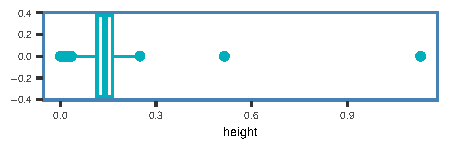
\includegraphics{ExecSum_files/figure-latex/unnamed-chunk-1-1} \end{center}

\hypertarget{analysis}{%
\section{Analysis}\label{analysis}}

\hypertarget{transformations}{%
\subsection{3.1 Transformations}\label{transformations}}

Prior to selecting an appropriate model, we must acknowledge that the
observed variables do not demonstrate a linear relationship with the
observed number of rings \emph{(Appendix 1)}, and we cannot consider
sexual maturity in its current state as a ternary factor. Due to the
nature of the observed curves, the ideal transformations for the
predictor variables were as follows: Log transformations for length,
diameter, and all the weights, and a square root transformation to
height. Transforming the predicted variable (rings) to the square root
of its logarithm proved ideal. Each predictor variable now adopts a
linear relationship with the predictive variable \emph{(Appendix 2)},
allowing for a linear regressive model to work appropriately.
Additionally, the sexual maturity factor was encoded using a contrast
matrix.

\hypertarget{model-selection}{%
\subsection{3.2 Model Selection}\label{model-selection}}

Having conducted our transformations, models could now be constructed.
Two models were constructed; one using forward stepping variable
selection, and the other using backward stepping variable selection.
Both of these models were evaluated considering their \(R^2\) and AIC
values. The produced models were remarkably similar in regard to the
above criteria, and the only notable difference between them is the
omission of diameter and length from the forward model. The produced
models are shown in the table below.

\begin{center}
\begin{tabular}{c c c c c}
    & Forward Model & & Backward Model & \\
    \hline
    Predictors & Estimates & p & Estimates & p\\
    \hline
    (Intercept) & 1.43 & $\textbf{<0.001}$ & 1.45 & $\textbf{<0.001}$\\
    log shell & 0.11 & $\textbf{<0.001}$ & 0.11 & $\textbf{<0.001}$\\
    log shucked & -0.19 & $\textbf{<0.001}$ & -0.19 & $\textbf{<0.001}$\\
    log whole & 0.19 & $\textbf{<0.001}$ & 0.20 & $\textbf{<0.001}$\\
    sex infant & -0.02 & $\textbf{<0.001}$ & -0.01 & $\textbf{<0.001}$\\
    log viscera & -0.03 & $\textbf{<0.001}$ & -0.02 & $\textbf{<0.001}$\\
    sqrt height & 0.13 & $\textbf{0.007}$ & 0.12 & $\textbf{0.012}$\\
    log diameter &  & & 0.07 & $\textbf{0.005}$\\
    log length &  & & -0.08 & $\textbf{0.005}$\\
    \hline
    Observations & 4175 &  & 1.45 & \\
    $R^2/R^2$ adjusted & 0.647 / 0.647 & & 0.648 / 0.647 & \\
    AIC & -10882.310 & & -10887.886 & \\
\end{tabular}
\end{center}

\newpage

\hypertarget{assumption-checking}{%
\subsection{3.3 Assumption Checking}\label{assumption-checking}}

\hypertarget{forward-residual-vs-fittedqq-plot}{%
\subsubsection{Forward Residual vs Fitted/QQ
Plot}\label{forward-residual-vs-fittedqq-plot}}

\begin{center}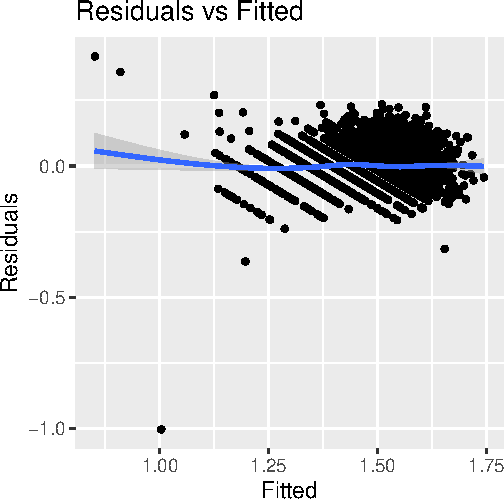
\includegraphics{ExecSum_files/figure-latex/unnamed-chunk-4-1} \end{center}

\hypertarget{backward-residual-vs-fittedqq-plot}{%
\subsubsection{Backward Residual vs Fitted/QQ
Plot}\label{backward-residual-vs-fittedqq-plot}}

\begin{center}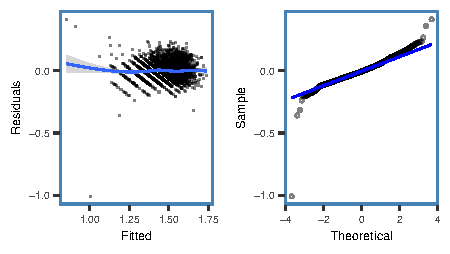
\includegraphics{ExecSum_files/figure-latex/unnamed-chunk-5-1} \end{center}

We must state and justify our assumptions - for both models - to
validate any inferences made in our results.

\begin{itemize}
\tightlist
\item
  \textbf{Linearity}: The residual plot displays no obvious curvature
  for either model, thus the linearity assumption is satisfied.
\item
  \textbf{Independence}: The data were collected across 5 different
  regions in the Tasman Sea \textit{(Appendix 3)}, with no systematic or
  intentional collection grouping. Granted these facts, there is no
  reason to believe there is any dependence between observations. Hence,
  independence can reasonably be assumed.
\item
  \textbf{Homoskedasticity}: For both models, the residuals do not
  appear to be fanning out or changing over the range of fitted values.
  Thus the constant error variance assumption is met.
\item
  \textbf{Normality}: The normality assumption is at least approximately
  satisfied. For the QQ plot of each model, the points are reasonably
  close to the diagonal line. Regardless, the sample size is large
  enough to rely upon the central limit theorem.
\end{itemize}

\hypertarget{results}{%
\section{Results}\label{results}}

Since the models constructed using the forward and backward approach
share the same adjusted \(R^2\), the Residual Mean Square Error (RMSE)
and Mean Absolute Error (MAE) were computed for each in order to
determine and justify the better model. Graphs are shown below.

\begin{center}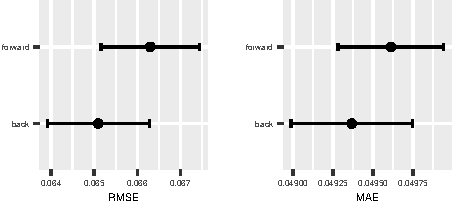
\includegraphics{ExecSum_files/figure-latex/unnamed-chunk-8-1} \end{center}

It is evident that the backward model is the better model, as it has a
lower RMSE and MAE. It is worth noting that the p-values for all the
original variables are statistically significant, excepting one of the
sexual maturity factors produced from the dummy coding contrast matrix.
The p-value for \texttt{sex\_f} was consistent with the null hypothesis
that the \textbf{gender} of the abalone is immaterial, while
\texttt{sex\_i} was significant, indicating that the sexual
\textbf{maturity} of the abalone was meaningful.

\par

It must be conceded that there is apparent multicollinearity within the
dataset \emph{(Appendix 4)}; which may reduce the precision of the
estimate coefficients and lessen the statistical power of the model.
This multicollinearity is to be expected. Living organisms tend to grow
physically as they age, with a rate that decreases over time. Naturally,
our measured values display that trend.

\par

It is a challenge to address multicollinearity within a data set where
all the variables are significant. The optimal solution is to omit
collinear variables which are already well represented by similar
measurements. In our specific case, this was a number of the weight
variables. The two more significant weight variables - according to the
standardized regression coefficients - were shucked weight and whole
weight;

\vspace{2mm}
\begin{tabular}{c c c c}
  log whole & log shucked & log viscera & log shell \\
  $1.4790451$ & $-1.5000279$ & $-0.1885621$ & $0.8269786$ \\
\hline
  log diam & log length & sqrt height & sex infant \\
  $0.19408468$ & $-0.19821088$ & $0.06175294$ & $-0.06326012$
\end{tabular}
\vspace{2mm}

Thus the viscera weight and shell weight were ignored in our final
model;

\begin{align*}
  \widehat{\sqrt{log(rings)}} &= 1.330 + 0.297 log(whole) -0.243 log(shucked)\\
  & + 0.153 log(diameter) -0.079 log(length)\\
  & + 0.205\sqrt{height}-0.013 Sex_{infant}
\end{align*}

Our model can predict the square root of the log of the number of rings
with 62.8\% explainable variance when using all the provided variables,
making for a respectable regressive model.

\hypertarget{discussion-and-conclusion}{%
\section{Discussion and Conclusion}\label{discussion-and-conclusion}}

We have constructed a model that will approximate an abalone's age from
easily measured attributes - a useful tool when monitoring large marine
ecosystems, where research time is far better spent collecting and
analysing observations than counting rings.

\hypertarget{limitations}{%
\subsection{5.1 Limitations}\label{limitations}}

\begin{itemize}
\tightlist
\item
  Our data only pertains to \emph{Haliotis Rubra}. The model does not
  account for species, and cannot claim to perform generally among
  Haliotes. Any conservational or environmental inferences are thus
  limited.
\item
  As noted above, there is high collinearity among the weight variables,
  and together this reduces the usefulness of each. It would perhaps be
  more profitable to forego one of these measurements in favour of
  another that would add more breadth to our profile of the abalone.
\item
  The data were only collected from waters surrounding Tasmania
  \emph{(Appendix 3)}. Although Blacklip Abalone \textbf{is} prevalent
  in these waters, they are found in coastal waters reaching all the way
  from lower NSW to lower WA. This restricts the usefulness of the
  model, since it can only be used with confidence for Abalone in
  Tasmanian waters - a portion of a much larger population.
\end{itemize}

\hypertarget{appendix}{%
\section{Appendix}\label{appendix}}

\textbf{Appendix 1: Correlation matrix of initial dataset}

\begin{center}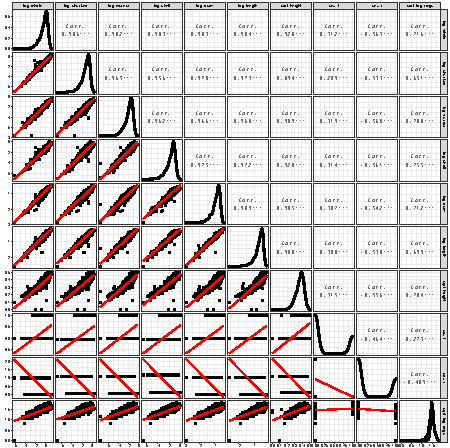
\includegraphics{ExecSum_files/figure-latex/unnamed-chunk-10-1} \end{center}

\textbf{Appendix 2: Correlation matrix of transformed variables}

\begin{center}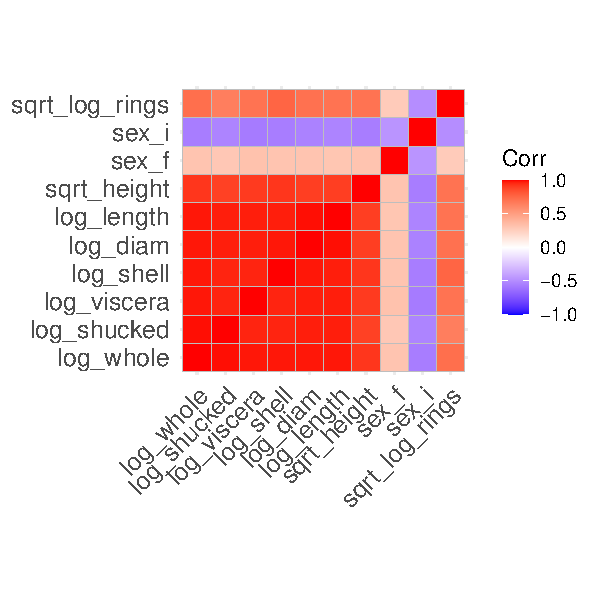
\includegraphics{ExecSum_files/figure-latex/unnamed-chunk-11-1} \end{center}

\textbf{Appendix 3: Data Collection Sites (\cite{article})}

\begin{figure}[H]
    \begin{center}
    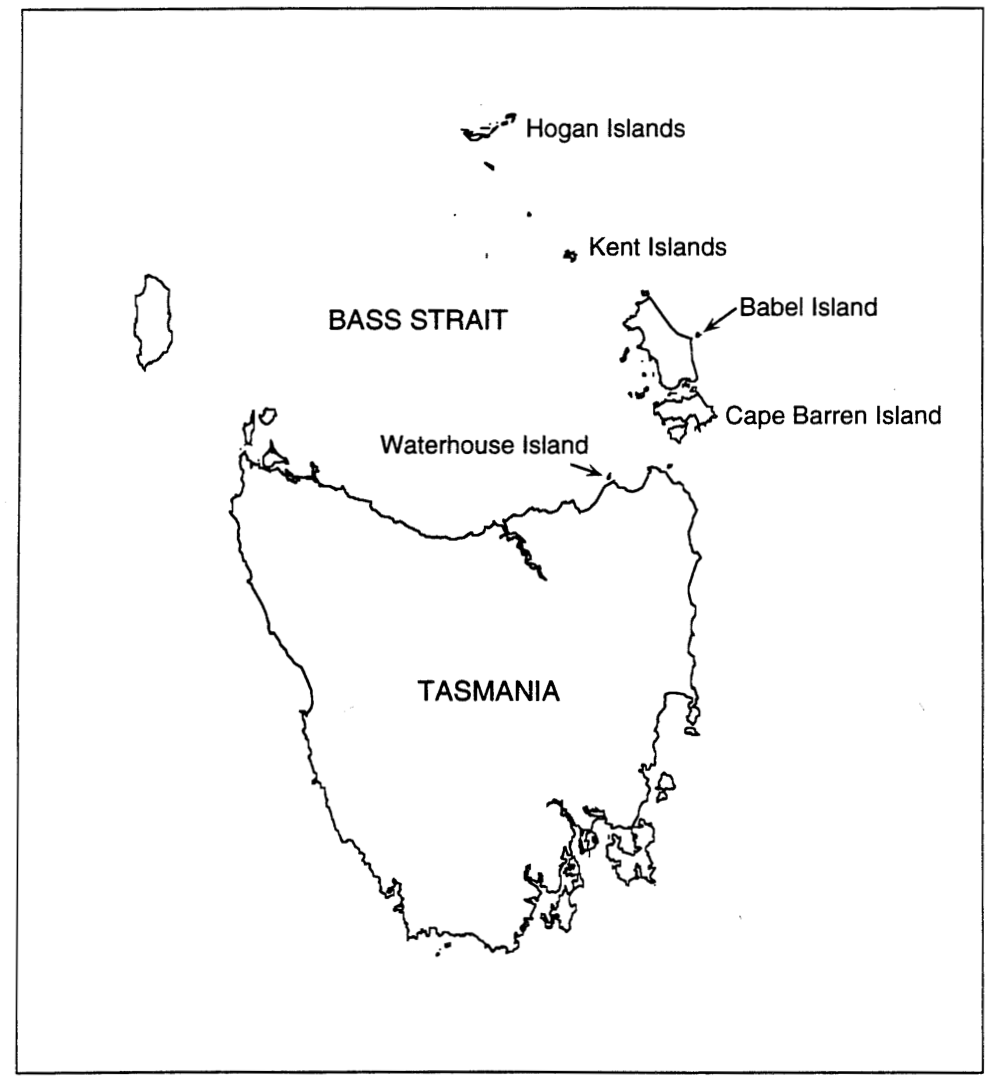
\includegraphics[width=0.35\textwidth, height=2in]{Independence} 
    \end{center}
\end{figure}

\newpage

\textbf{Appendix 4: Correlation Matrix}

\begin{center}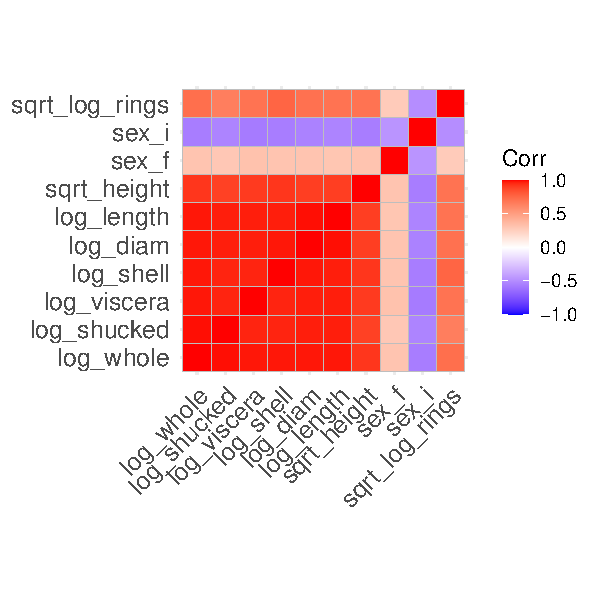
\includegraphics{ExecSum_files/figure-latex/unnamed-chunk-12-1} \end{center}

%\showmatmethods

\pnasbreak 



\begin{thebibliography}{3}
\newcommand{\enquote}[1]{``#1''}
\providecommand{\natexlab}[1]{#1}
\providecommand{\url}[1]{\texttt{#1}}
\providecommand{\urlprefix}{URL }
\expandafter\ifx\csname urlstyle\endcsname\relax
  \providecommand{\doi}[1]{doi:\discretionary{}{}{}#1}\else
  \providecommand{\doi}{doi:\discretionary{}{}{}\begingroup
  \urlstyle{rm}\Url}\fi
\providecommand{\eprint}[2][]{\url{#2}}



\bibitem[{Allaire \emph{et~al.}(2017)Allaire, {R Foundation}, Wickham, {Journal
  of Statistical Software}, Xie, Vaidyanathan, {Association for Computing
  Machinery}, Boettiger, {Elsevier}, Broman, Mueller, Quast, Pruim, Marwick,
  Wickham, Keyes, and Yu}]{CRAN:rticles}
Allaire J, {R Foundation}, Wickham H, {Journal of Statistical Software}, Xie Y,
  Vaidyanathan R, {Association for Computing Machinery}, Boettiger C,
  {Elsevier}, Broman K, Mueller K, Quast B, Pruim R, Marwick B, Wickham C,
  Keyes O, Yu M (2017).
\newblock \emph{rticles: Article Formats for R Markdown}.
\newblock R package version 0.4.1,
  \urlprefix\url{https://CRAN.R-project.org/package=rticles}.

\bibitem[{MacFarlane(2017)}]{pandoc}
MacFarlane J (2017).
\newblock \emph{Pandoc: A Universal Document Converter}.
\newblock Version 1.19.2.1, \urlprefix\url{http://pandoc.org}.

\bibitem[{Xie(2017)}]{CRAN:knitr}
Xie Y (2017).
\newblock \emph{knitr: A General-Purpose Package for Dynamic Report Generation
  in R}.
\newblock R package version 1.17, \urlprefix\url{https://yihui.name/knitr/}.

\bibitem[{Karl~W. Broman(2015)}]{b}
Karl~W. Broman (2015).
\newblock R/qtlcharts: interactive graphics for quantitative trait locus
  mapping.
\newblock {\emph Genetics}, 199:359--361, \urlprefix\url{http://www.genetics.org/content/genetics/199/2/359.full.pdf}.

\bibitem[{Dheeru Dua and Casey Graff(2017)}]{Dua:2019}
Dheeru Dua and Casey Graff (2017).
\newblock {UCI} machine learning repository, \urlprefix\url{https://archive.ics.uci.edu/ml/datasets/abalone}.

\bibitem[{Dirk Eddelbuettel and James~Joseph Balamuta(August 2017)}]{PeerJ:Rcpp}
Dirk Eddelbuettel and James~Joseph Balamuta (August 2017).
\newblock Extending \textit{R} with \textit{C++}: A brief introduction to
  \textit{Rcpp}.
\newblock {\emph PeerJ Preprints}, 5:e3188v1, \urlprefix \url{https://doi.org/10.7287/peerj.preprints.3188v1}.

\bibitem[{Max Kuhn(2020)}]{d}
Max Kuhn (2020).
\newblock {\emph caret: Classification and Regression Training}.
\newblock R package version 6.0-86, \urlprefix \url{https://CRAN.R-project.org/package=caret}.

\bibitem[{Daniel Lüdecke(2020)}]{e}
Daniel Lüdecke (2020).
\newblock {\emph sjPlot: Data Visualization for Statistics in Social Science}.
\newblock R package version 2.8.6, \urlprefix \url{https://CRAN.R-project.org/package=sjPlot}.

\bibitem[{Warwick \emph{et~al.}(1994) Nash, T.L. Sellers, S.R. Talbot, A.J. Cawthorn, and W.B. Ford}]{article}
Warwick Nash, T.L. Sellers, S.R. Talbot, A.J. Cawthorn, and W.B. Ford (1994).
\newblock 7he population biology of abalone (haliotis species) in tasmania.
  i. blacklip abalone (h. rubra) from the north coast and islands of bass
  strait.
\newblock {\emph Sea Fisheries Division, Technical Report No}, 48, \urlprefix \url{https://www.researchgate.net/publication/287546509_7he_Population_Biology_of_Abalone_Haliotis_species_in_Tasmania_I_Blacklip_Abalone_H_rubra_from_the_North_Coast_and_Islands_of_Bass_Strait}

\bibitem[{Barret Schloerke, Di~Cook, Joseph Larmarange, Francois Briatte, Moritz Marbach,
  Edwin Thoen, Amos Elberg, and Jason Crowley (2020)}]{c}
Barret Schloerke, Di~Cook, Joseph Larmarange, Francois Briatte, Moritz Marbach,
  Edwin Thoen, Amos Elberg, and Jason Crowley(2020).
\newblock {\emph GGally: Extension to 'ggplot2'}.
\newblock R package version 2.0.0, \urlprefix \url{https://CRAN.R-project.org/package=GGally}.

\bibitem[{Taiyun Wei and Viliam Simko(2017)}]{corrplot2017}
Taiyun Wei and Viliam Simko (2017).
\newblock {\emph R package "corrplot": Visualization of a Correlation Matrix}.
\newblock (Version 0.84), \urlprefix \url{https://github.com/taiyun/corrplot}.

\bibitem[{Hadley Wickham, Mara Averick, Jennifer Bryan, Winston Chang, Lucy~D'Agostino
  McGowan, Romain François, Garrett Grolemund, Alex Hayes, Lionel Henry, Jim
  Hester, Max Kuhn, Thomas~Lin Pedersen, Evan Miller, Stephan~Milton Bache,
  Kirill Müller, Jeroen Ooms, David Robinson, Dana~Paige Seidel, Vitalie
  Spinu, Kohske Takahashi, Davis Vaughan, Claus Wilke, Kara Woo, and Hiroaki
  Yutani(2019).}]{a}
Hadley Wickham, Mara Averick, Jennifer Bryan, Winston Chang, Lucy~D'Agostino
  McGowan, Romain François, Garrett Grolemund, Alex Hayes, Lionel Henry, Jim
  Hester, Max Kuhn, Thomas~Lin Pedersen, Evan Miller, Stephan~Milton Bache,
  Kirill Müller, Jeroen Ooms, David Robinson, Dana~Paige Seidel, Vitalie
  Spinu, Kohske Takahashi, Davis Vaughan, Claus Wilke, Kara Woo, and Hiroaki
  Yutani (2019).
\newblock Welcome to the {tidyverse}.
\newblock {\emph Journal of Open Source Software}, 4(43):1686.

\end{thebibliography}

\end{document}

